%----------------------------------------------------------------------------------------
%	PACKAGES AND OTHER DOCUMENT CONFIGURATIONS
%----------------------------------------------------------------------------------------

\documentclass[landscape,a0paper,fontscale=0.5]{baposter} % Adjust the font scale/size here

\usepackage{graphicx} % Required for including images
\graphicspath{{figures/}} % Directory in which figures are stored

\usepackage{amsmath} % For typesetting math
\usepackage{amssymb} % Adds new symbols to be used in math mode

\usepackage{booktabs} % Top and bottom rules for tables
\usepackage{enumitem} % Used to reduce itemize/enumerate spacing
\usepackage{palatino} % Use the Palatino font
\usepackage[font=small,labelfont=bf]{caption} % Required for specifying captions to tables and figures

\usepackage{multicol} % Required for multiple columns
\setlength{\columnsep}{1.5em} % Slightly increase the space between columns
\setlength{\columnseprule}{0mm} % No horizontal rule between columns

\usepackage{tikz} % Required for flow chart
\usetikzlibrary{shapes,arrows} % Tikz libraries required for the flow chart in the template

\newcommand{\compresslist}{ % Define a command to reduce spacing within itemize/enumerate environments, this is used right after \begin{itemize} or \begin{enumerate}
\setlength{\itemsep}{1pt}
\setlength{\parskip}{0pt}
\setlength{\parsep}{0pt}
}

\definecolor{MRGGreen}{rgb}{0, 0.350, 0.200}

\newenvironment{ColFigure}
  {\par\medskip\noindent\minipage{\linewidth}}
  {\endminipage\par\medskip}


\begin{document}

\begin{poster}
{
headerborder=closed, % Adds a border around the header of content boxes
colspacing=1em, % Column spacing
bgColorOne=MRGGreen, % Background color for the gradient on the left side of the poster
bgColorTwo=MRGGreen, % Background color for the gradient on the right side of the poster
borderColor=MRGGreen, % Border color
headerColorOne=black, % Background color for the header in the content boxes (left side)
headerColorTwo=MRGGreen, % Background color for the header in the content boxes (right side)
headerFontColor=MRGGreen, % Text color for the header text in the content boxes
boxColorOne=white, % Background color of the content boxes
textborder=roundedleft, % Format of the border around content boxes, can be: none, bars, coils, triangles, rectangle, rounded, roundedsmall, roundedright or faded
eyecatcher=true, % Set to false for ignoring the left logo in the title and move the title left
headerheight=0.1\textheight, % Height of the header
headershape=roundedright, % Specify the rounded corner in the content box headers, can be: rectangle, small-rounded, roundedright, roundedleft or rounded
headerfont=\Large\bf\textsc, % Large, bold and sans serif font in the headers of content boxes
%textfont={\setlength{\parindent}{1.5em}}, % Uncomment for paragraph indentation
linewidth=2pt % Width of the border lines around content boxes
}
%----------------------------------------------------------------------------------------
%	TITLE SECTION 
%----------------------------------------------------------------------------------------
%
{
\includegraphics[height=4em]{graphics/logo.jpg}} % First university/lab logo on the left
{\bf\textsc{Unnecessarily Complicated Research Title}\vspace{0.5em}} % Poster title
{\textsc{\{ John Smith, James Smith and Jane Smith \} \hspace{12pt} University and Department Name}} % Author names and institution
{
\includegraphics[height=4em]{graphics/logo.jpg}} % Second university/lab logo on the right


%----------------------------------------------------------------------------------------
%	Objectives
%----------------------------------------------------------------------------------------

\headerbox{Objectives}{name=objective,column=0,row=0,span=2}{
\begin{multicols}{2}
\vspace{1em}
Probabilistic programming language and Bayesian inference
engine Stan supports general model specification
and uses dynamic HMC for fully Bayesian
analysis \cite{carpenter_stan_2017}. Torsten is a library of Stan functions that
simplifies pharmacometric modeling and
extends the range of models that may be implemented
\cite{Torsten}. To improve the performance of Bayesian inference of population models,
we designed a multilevel parallel scheme that combines
a cross-chain warmup algorithm
with within-chain parallelisation and
demonstrated that this approach significantly improves large
PKPD model simulation efficiency.

% With increasing adoption of Bayesian inference to
% pharmacometric(PMX) modeling, it has become evident that
% high-performance computing(HPC) must be utilized for large-scale
% models to be accessible, and inference framework based on Markov Chain
% Monte Carlo(MCMC) must improve efficiency through multiple
% channels. For example, probabilistic programming language Stan \cite{carpenter_stan_2017}
% uses efficient samplers such as the No-U-Turn
% Sampler(NUTS) \cite{hoffman_no-u-turn_2014}, and provide \texttt{\texttt{map\_rect}} functions
% to parallelize expensive likelihood evaluation.

% The scope of the work presented here is to improve Bayesian inference
% efficiency of population models. The work is based on Torsten
% \cite{Torsten}, a library of Stan functions that
% simplifies PMX modeling and
% extends the range of models that may be implemented. We address two
% aspects of the efficiency problem. First, we propose a dynamic warmup
% approach, as an alternative to current Stan's warmup where a fixed
% number(default 1000) of iterations are performed. Second, we combine
% the new warmup algorithm with existing within-chain parallelization
% functionality of Torsten \cite{torsten_pmx_group} to formulate a \emph{multilevel} parallel method
% that utilizes dynamic warmup \emph{and} within-chain parallelism to speed
% up simulation.
\end{multicols}
\vspace{0.5em}
}

%----------------------------------------------------------------------------------------
%	Cross-chain
%----------------------------------------------------------------------------------------

\headerbox{Cross-chain warmup}{name=warmup,column=0,span=2,below=objective,bottomaligned=conclusion}{
\begin{multicols}{2}
\vspace{1em}
The standard practice of Stan is to perform a fixed number of warmup
iterations. With this practice, the efficacy of the warmup is unknown
\emph{a priori} and often warmup is unncessarily long as user oversubscribe warmup iterations.
The proposed warmup algorithm tries to avoid this by checking potential scale reduction
coefficients (\(\hat{R}\)) and effective sample sizes (ESS)
\cite{vehtari_rank-normalization_2019} . Specifically, for warmup we propose
\begin{ColFigure}
 \centering
 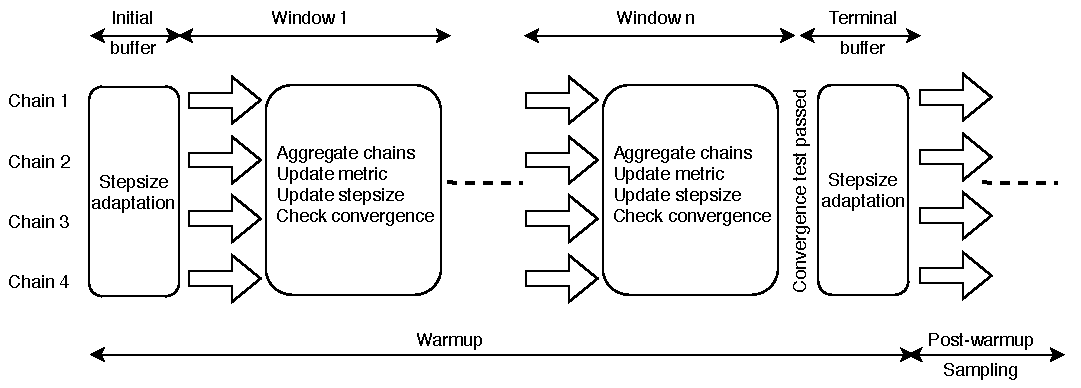
\includegraphics[width=\linewidth]{figure/cross_chain_diagram.pdf}
 \captionof{figure}{my caption of the figure}
\end{ColFigure}

\begin{enumerate}
\item Given a fixed window size \(w\)(default 100 iterations), the sampler iterates during warmup with stepsize adapted as in regular warmup runs.
\item At the end of a window, joint posterior probability from all the
  chains are aggregated and used to calculate corresponding \(\hat{R}\) and ESS. 
For example, with default window size \(w=100\), when warmup reaches iteration 300, we calculate
\(\hat{R}^i\) and \(\text{ESS}^i\) for \(i=1, 2, 3\), so that
\(\hat{R}^1\) and \(\text{ESS}^1\) are based on warmup iteration 1 to 300,
\(\hat{R}^2\) and \(\text{ESS}^2\) are based on warmup iteration 101 to 300,
and
\(\hat{R}^3\) and \(\text{ESS}^3\) are based on warmup iteration 201 to 300.

\item At the end of window \(n\), with predefined target value
  \(\hat{R}^{0}\) and ESS\(^{0}\), from \({1, \dots, n}\),  we select
  \(j\) with maximum 
$\text{ESS}^j$,
and a new metric is calculated by aggregating samples from
corresponding windows.
If, in addition, \(j\) satisfies $\hat{R}^j < \hat{R}^0$ and $\text{ESS}^j > \text{ESS}^0$,
the warmup is considered complete(\emph{converges}). Otherwise warmup continues until
the end of the next window and step 2-3 are repeated.
\end{enumerate}
Unlike current warmup scheme, the above proposal requires
communication among the chains, hence we call it \emph{cross-chain warmup}.

In benchmark, the above warmup scheme is compared against standard Stan warmup(1000
iterations) on several models for their
\begin{ColFigure}
\centering
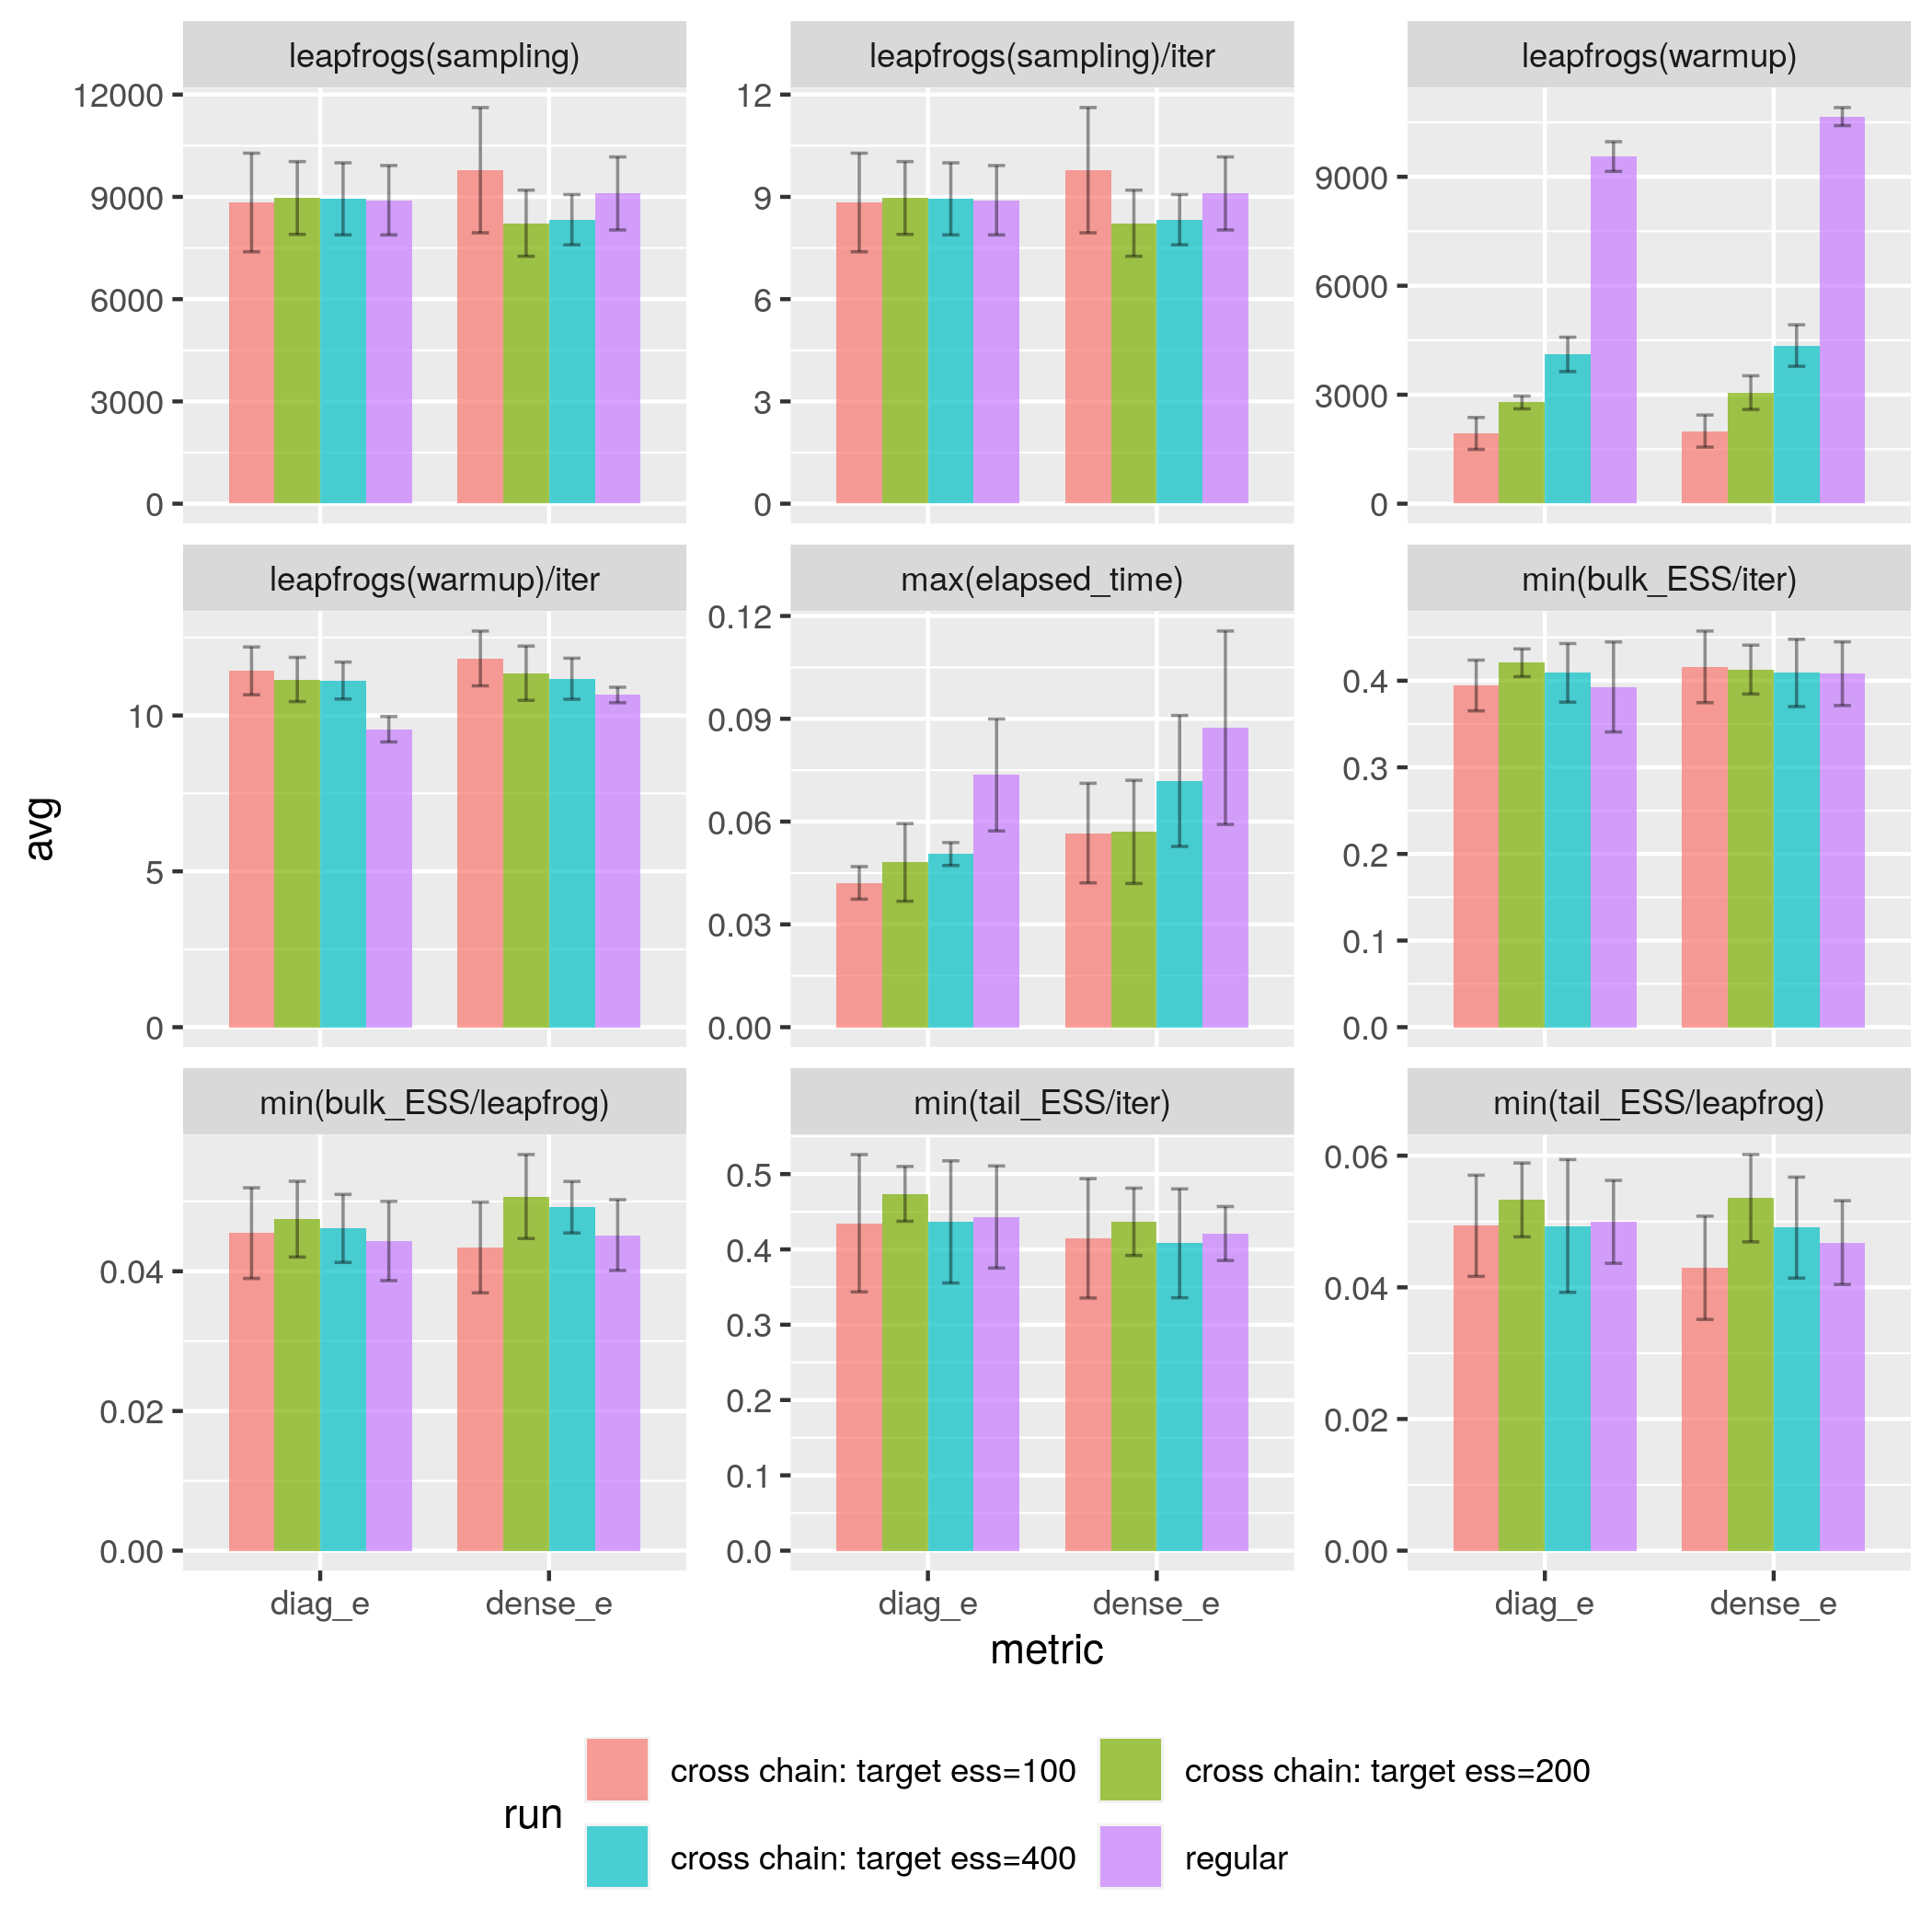
\includegraphics[width=0.8\linewidth]{./figure/cross_chain_ess_effect_eight_schools.png}
\captionof{figure}{Cross-chain warmup performance comparison: eight schools model}
\end{ColFigure}

\begin{ColFigure}
\centering
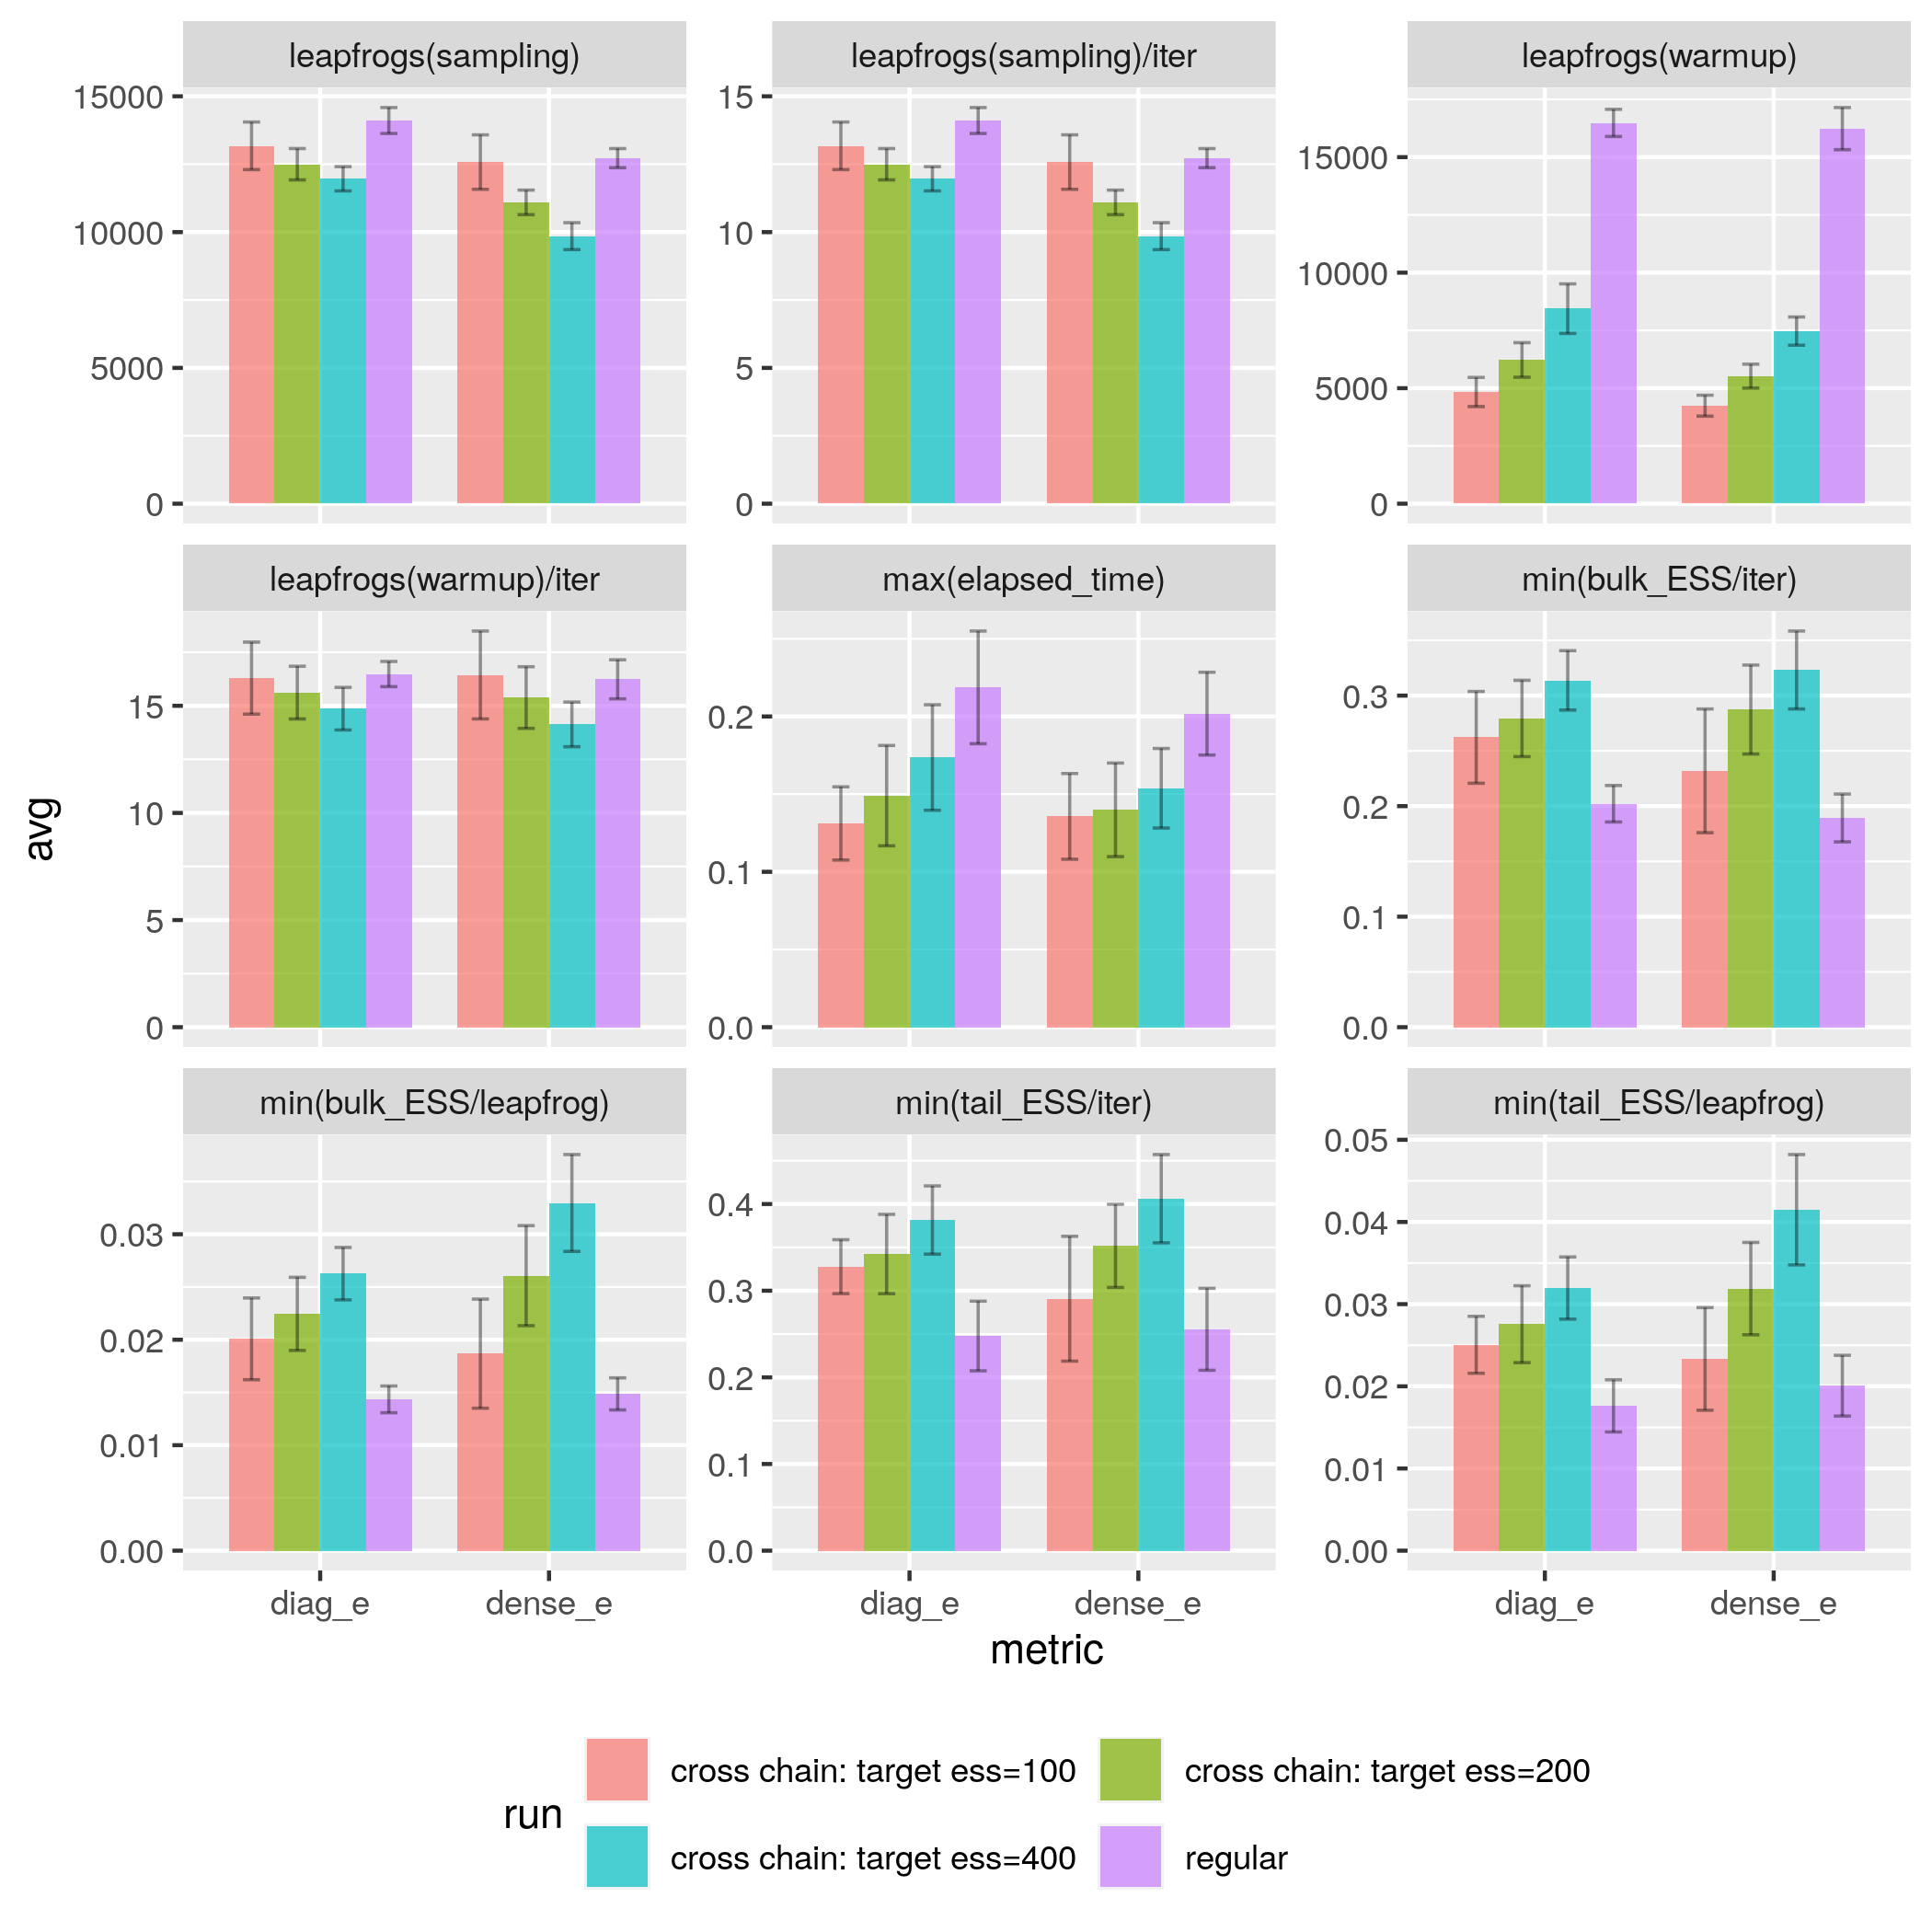
\includegraphics[width=0.8\linewidth]{./figure/cross_chain_ess_effect_sblrc-blr.png}
\caption{Cross-chain warmup performance comparison: garch-garch11 model}
\end{ColFigure}

\begin{ColFigure}
\centering
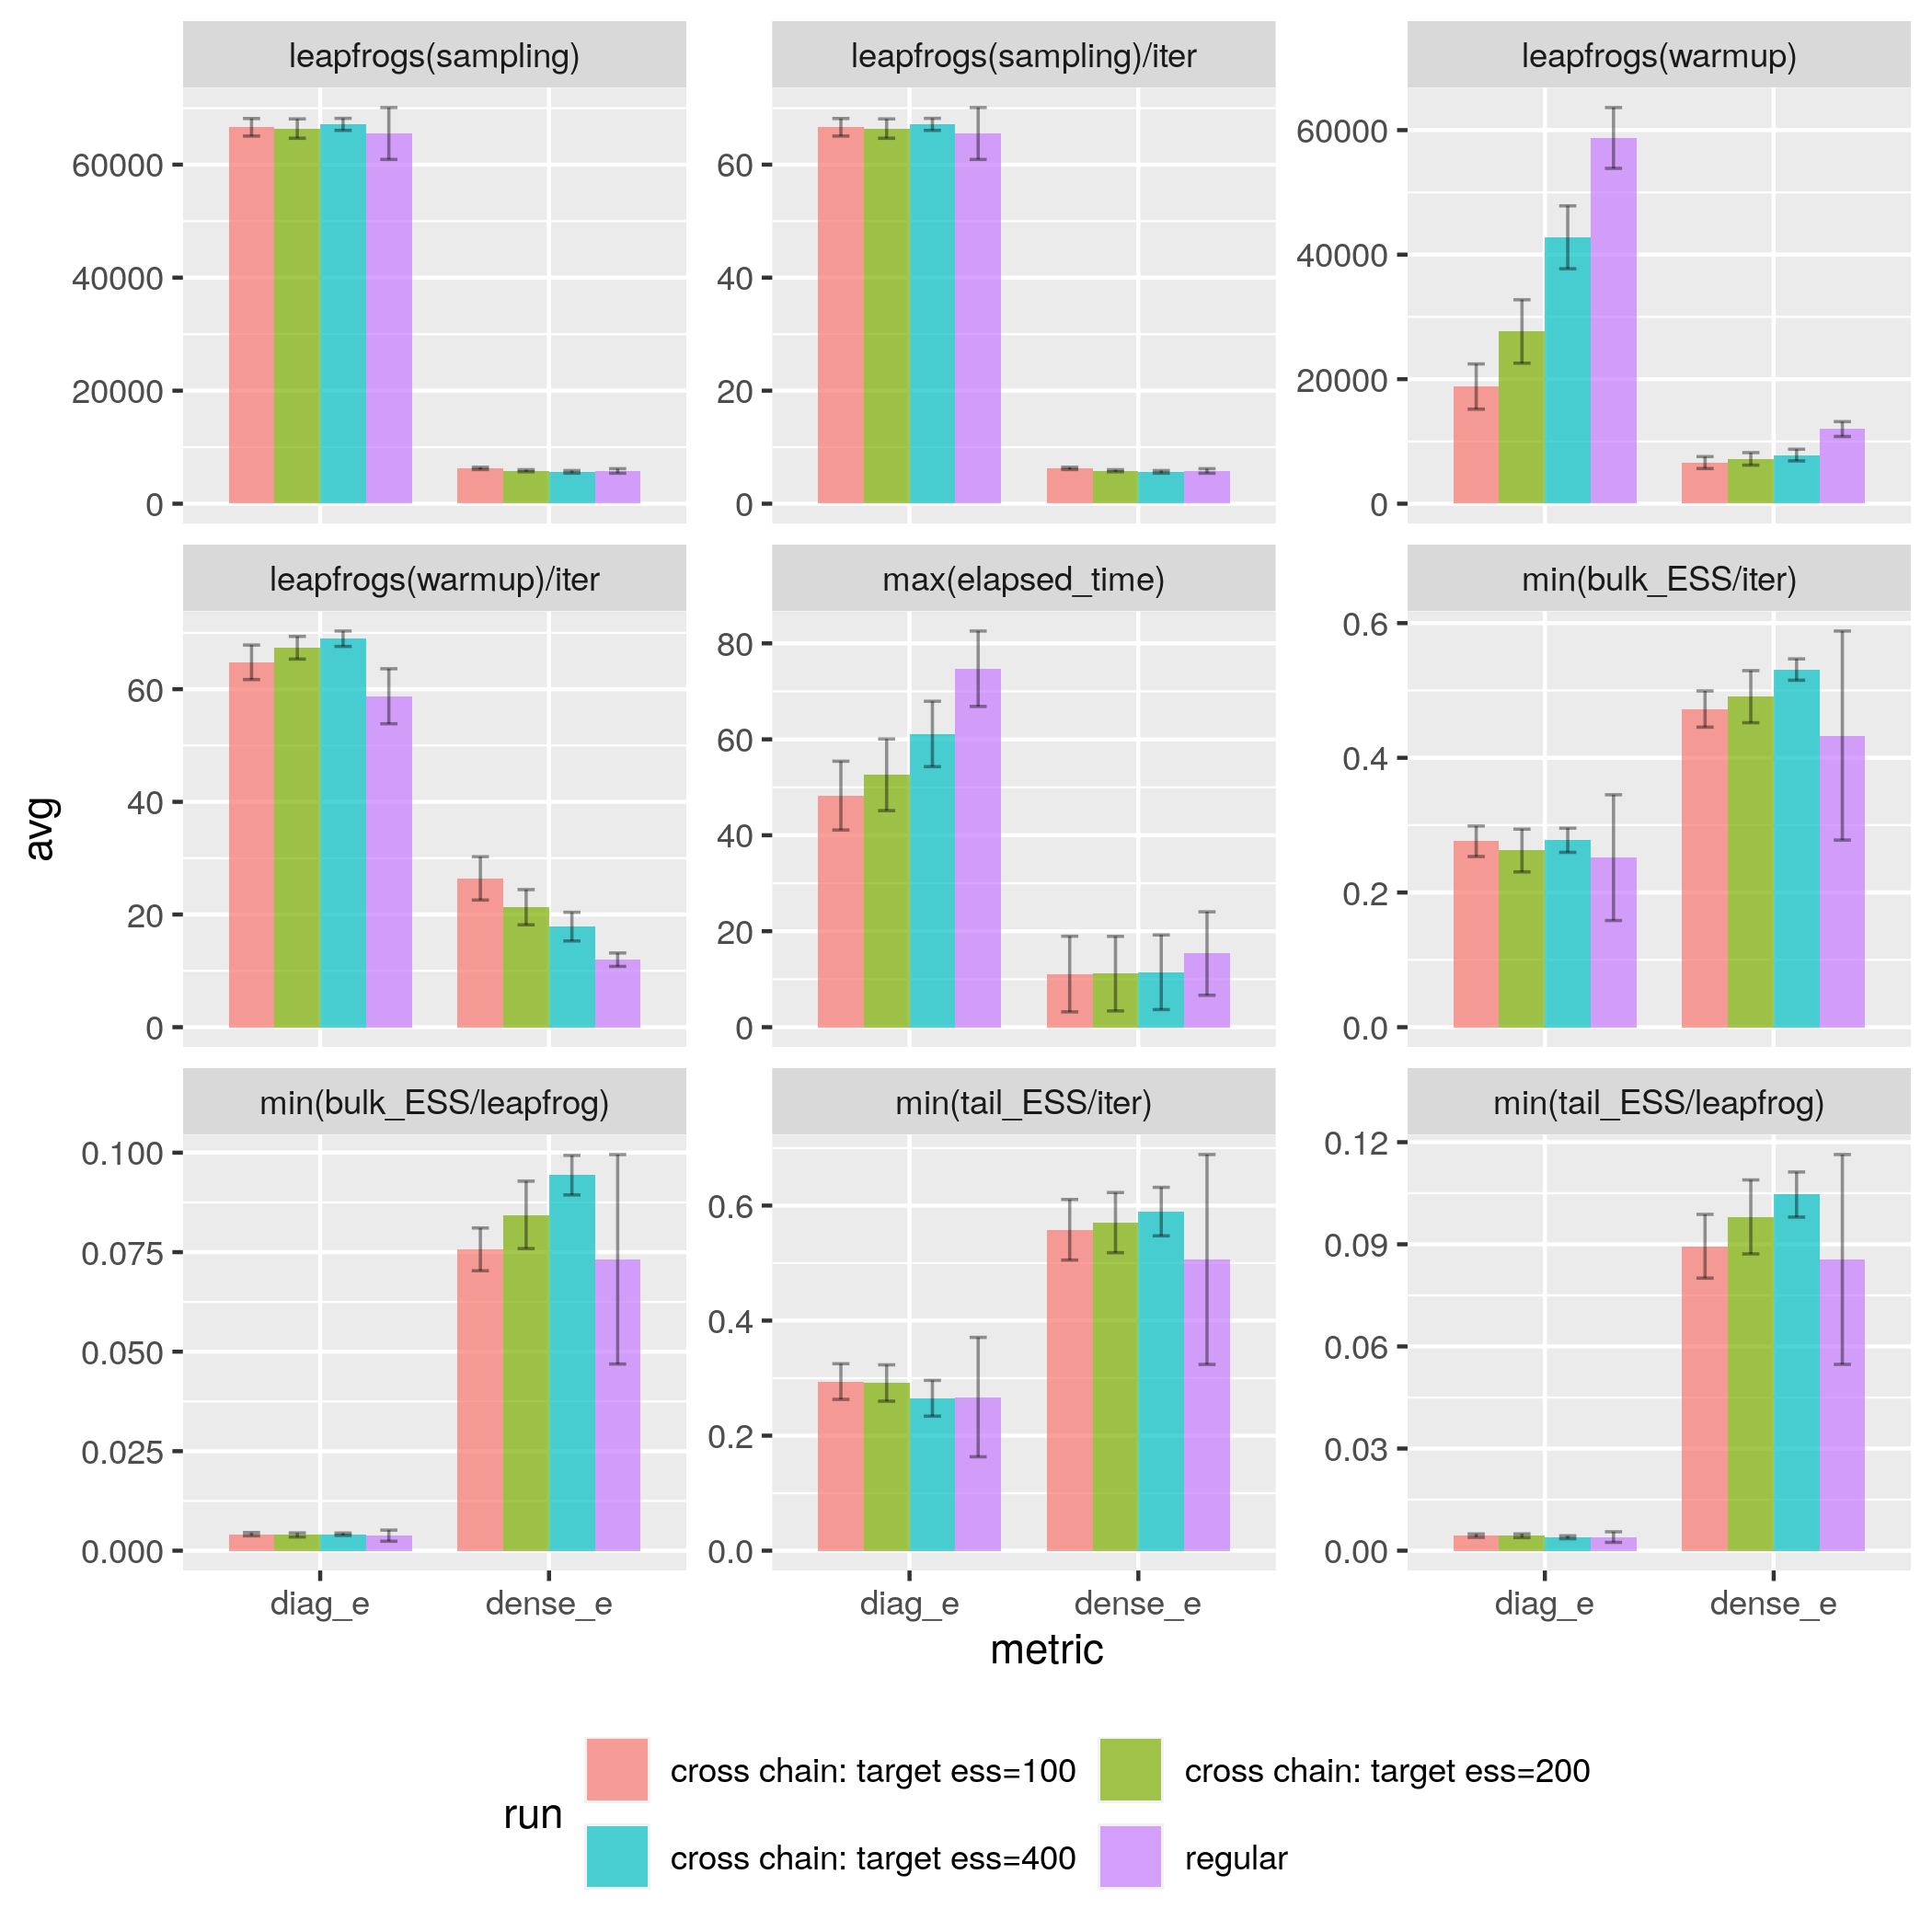
\includegraphics[width=0.8\linewidth]{./figure/cross_chain_ess_effect_sir.png}
\caption{Cross-chain warmup performance comparison: SIR model}
\end{ColFigure}

\begin{center}
\begin{tabular}{l}
\hline
total number of leapfrog integration steps in warmup \\
total number of leapfrog integration steps in sampling \\
number of leapfrog integration steps in per each warmup iteration \\
number of leapfrog integration steps in per each sampling iteration \\
minimum ESS\(_{\text{bulk}}\) per iteration \\
minimum ESS\(_{\text{tail}}\) per iteration \\
minimum ESS\(_{\text{bulk}}\) per leapfrog step \\
minimum ESS\(_{\text{tail}}\) per leapfrog step \\
maximum wall time
\hline
\end{tabular}
\end{center}
Each setup is run with 10 PRNG seeds and the quantities' average(barplot)
and standard deviation(error bar) are shown. All wall time are in seconds.

% \begin{ColFigure}
% \centering
% 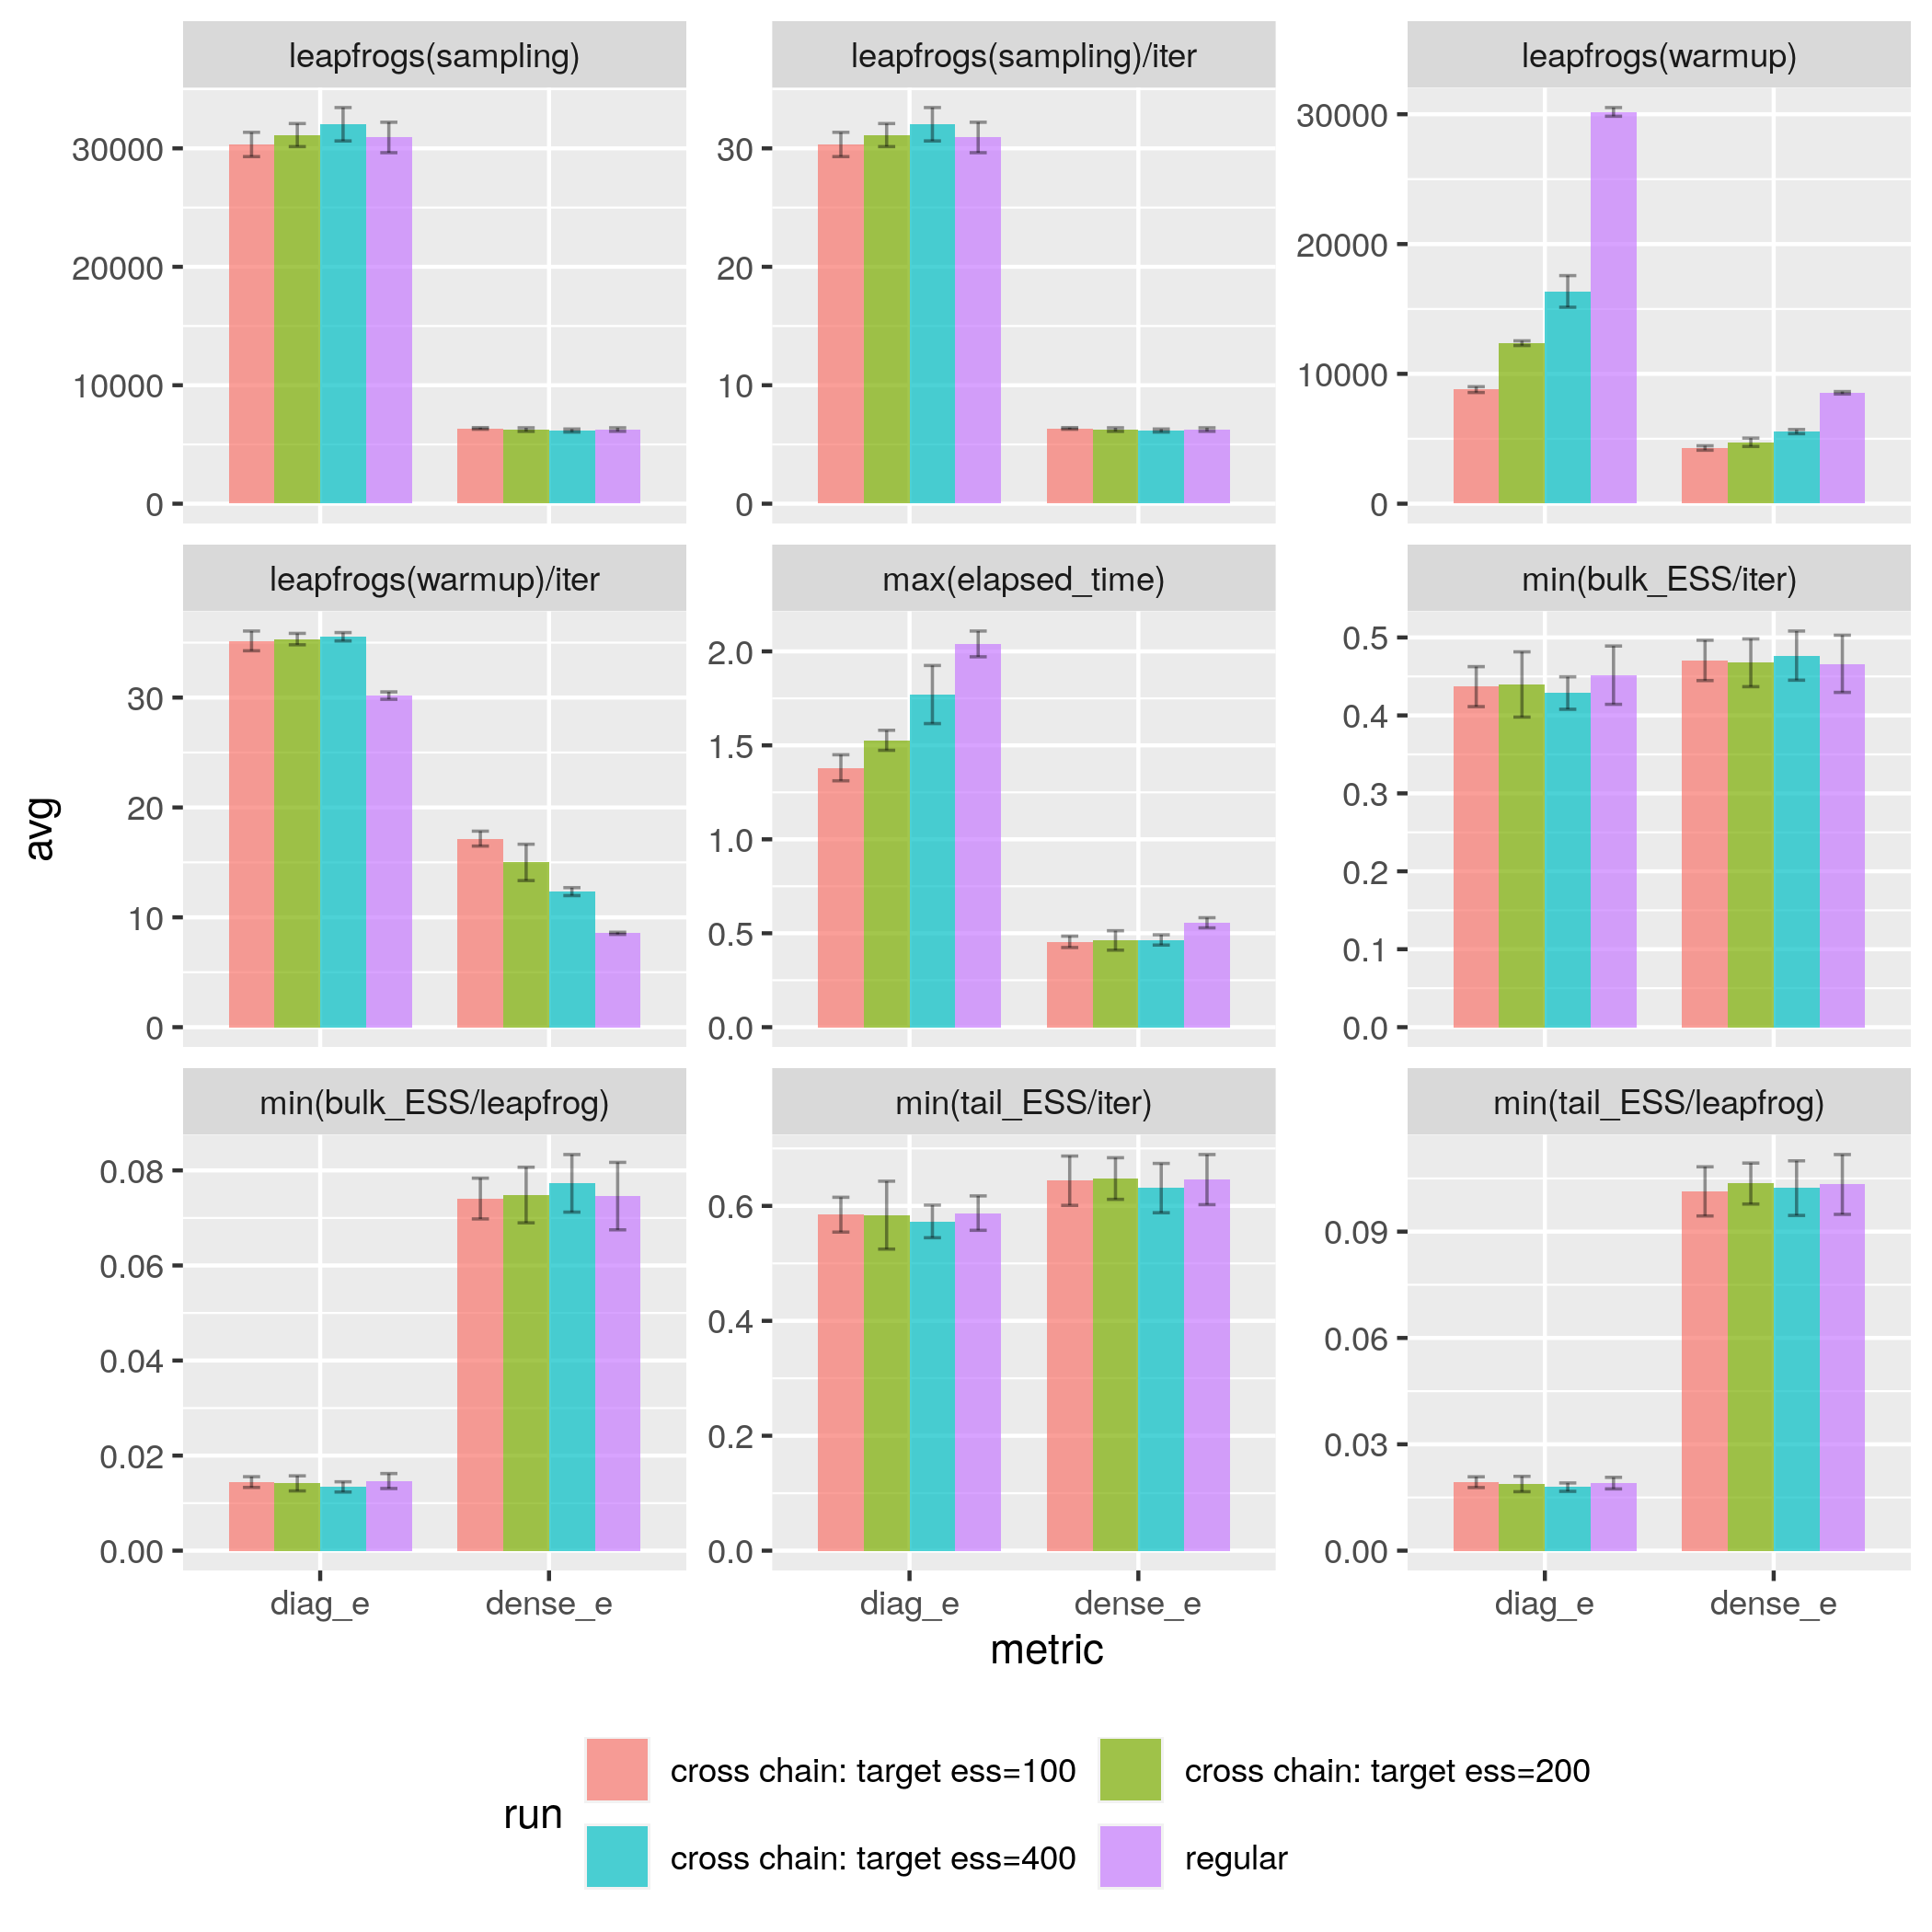
\includegraphics[width=0.7\linewidth]{./figure/cross_chain_ess_effect_arK.png}
% \caption{Cross-chain warmup performance comparison: arK model}
% \end{ColFigure}


% \begin{ColFigure}
% \centering
% 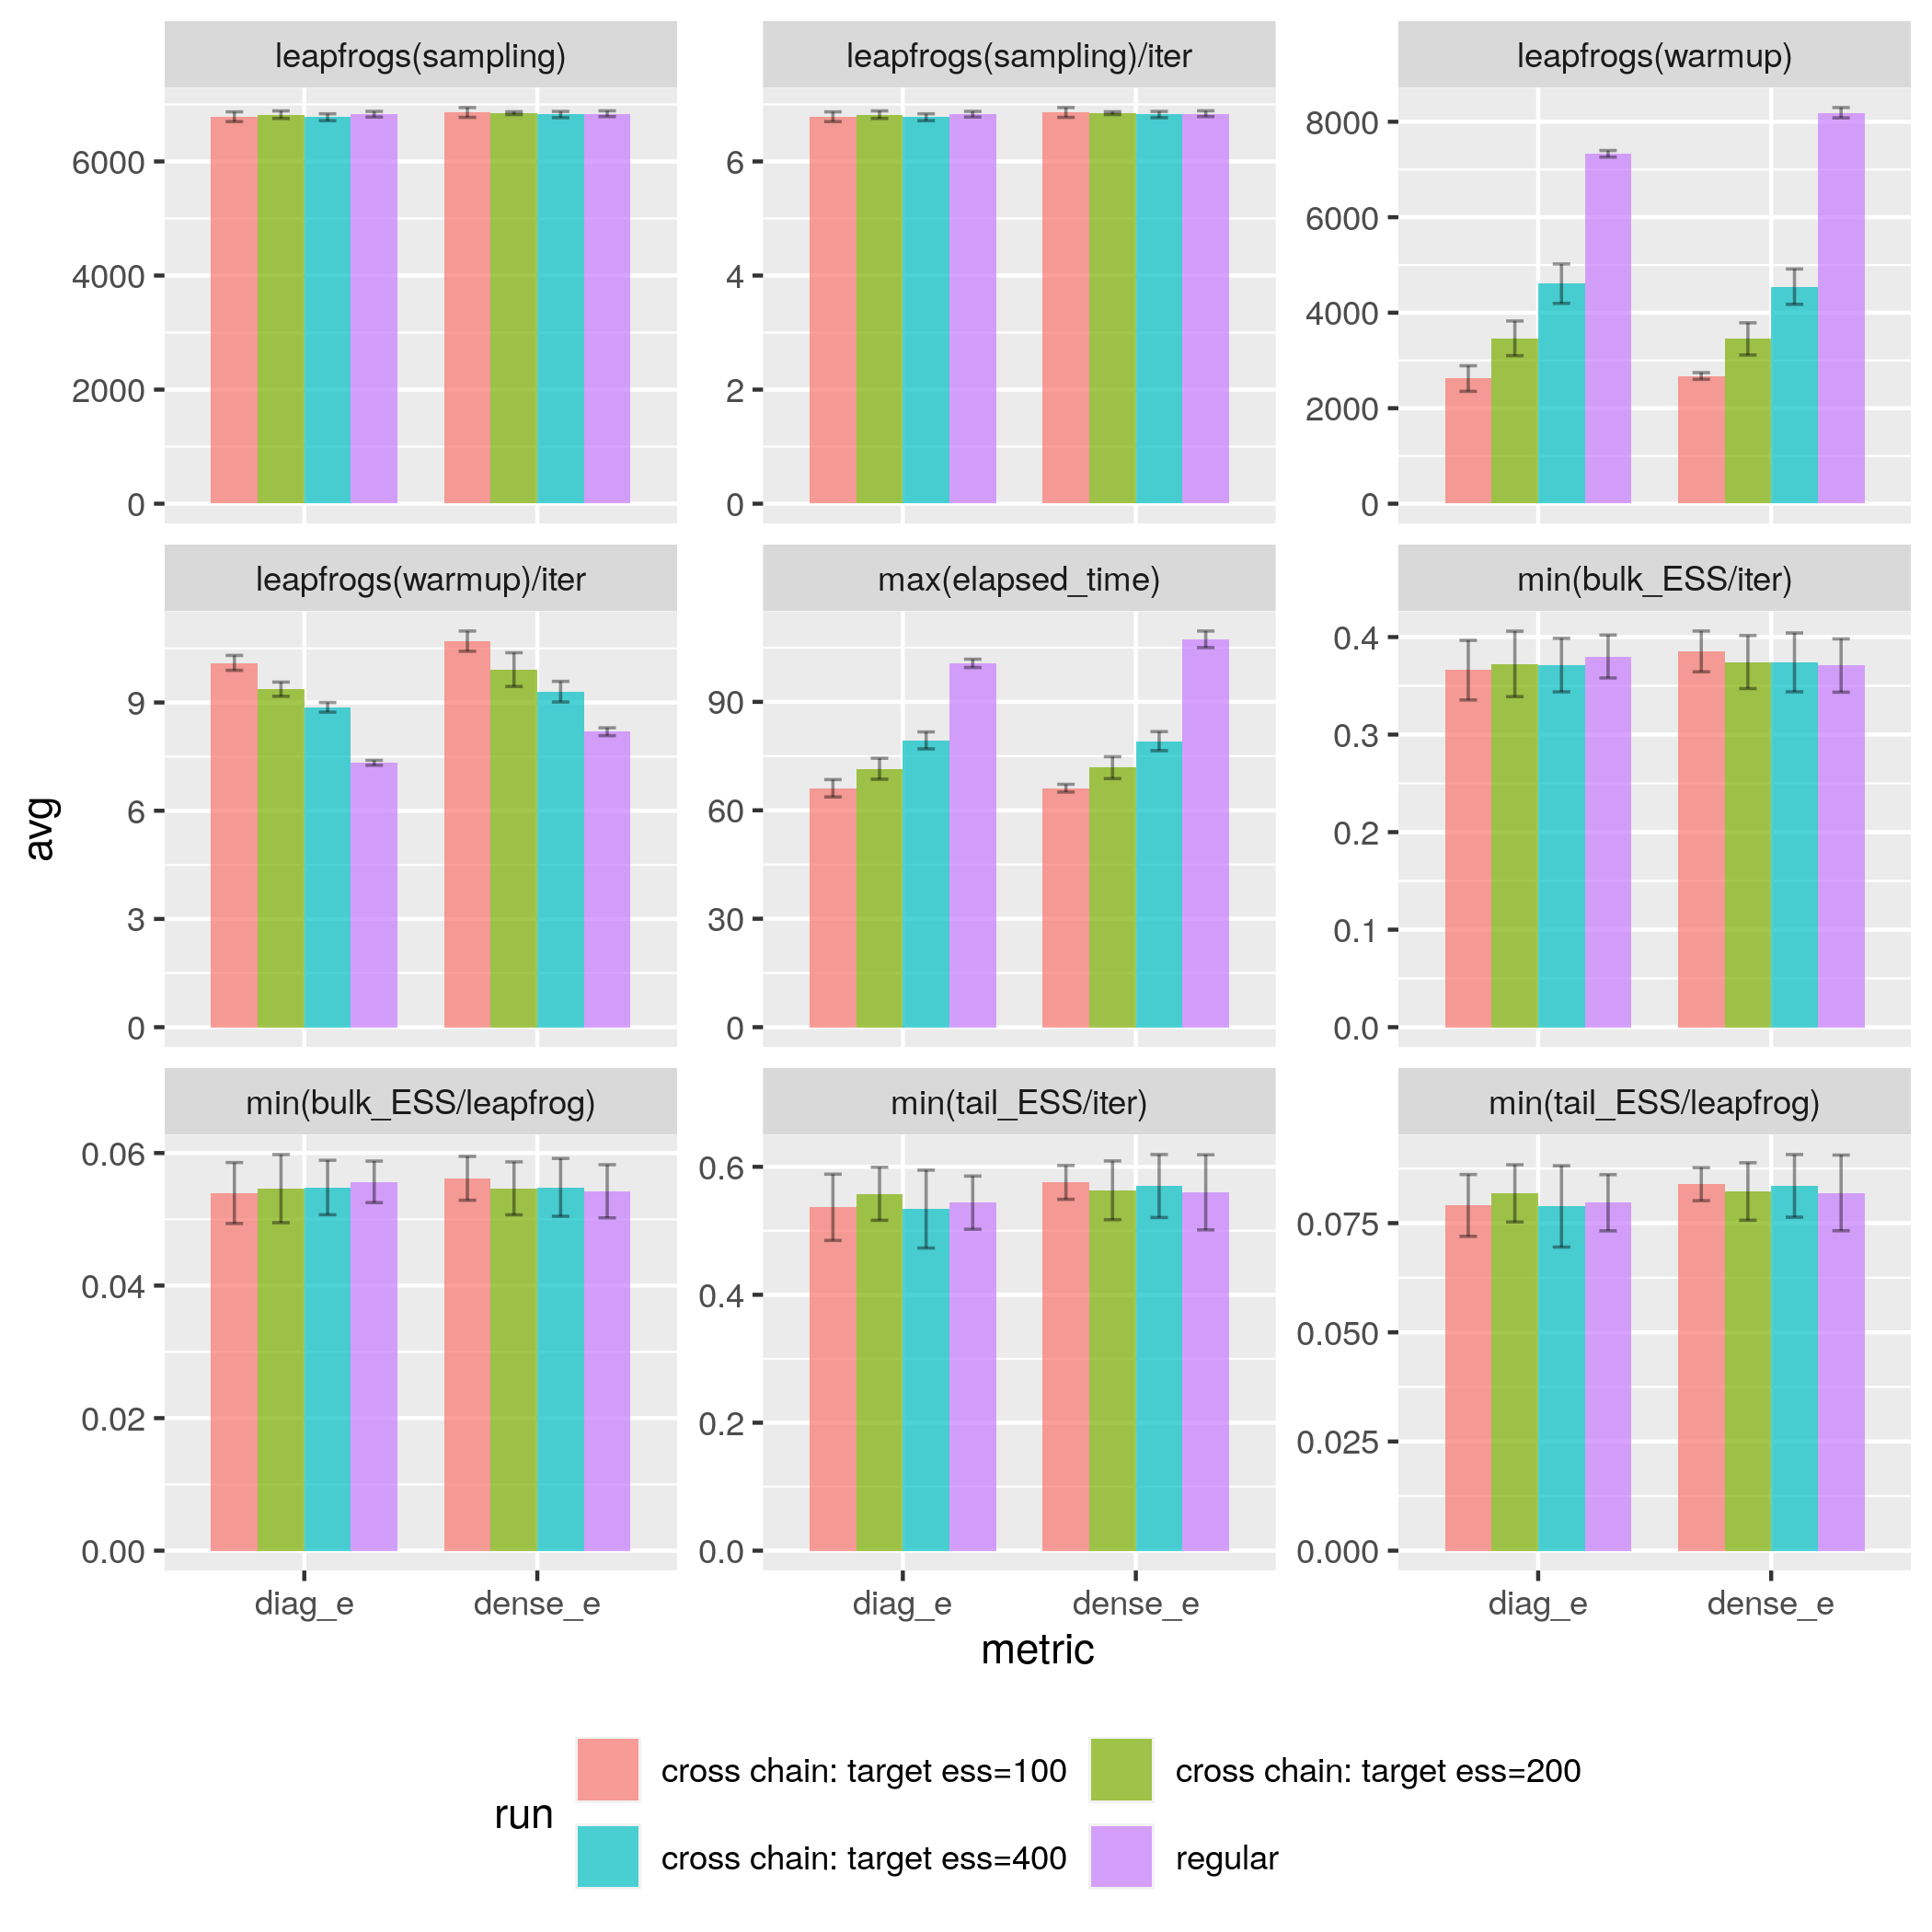
\includegraphics[width=0.7\linewidth]{./figure/cross_chain_ess_effect_chem.png}
% \caption{Cross-chain warmup performance comparison: chemical reaction model}
% \end{ColFigure}

\end{multicols}
}

%----------------------------------------------------------------------------------------
%	multilevel: method
%----------------------------------------------------------------------------------------

\headerbox{Multilevel parallelization: cross-chain warmup + within-chain parallelization}{name=multilevel,column=2,span=2,row=0}{

\begin{multicols}{2}
\vspace{1em}

\begin{center}
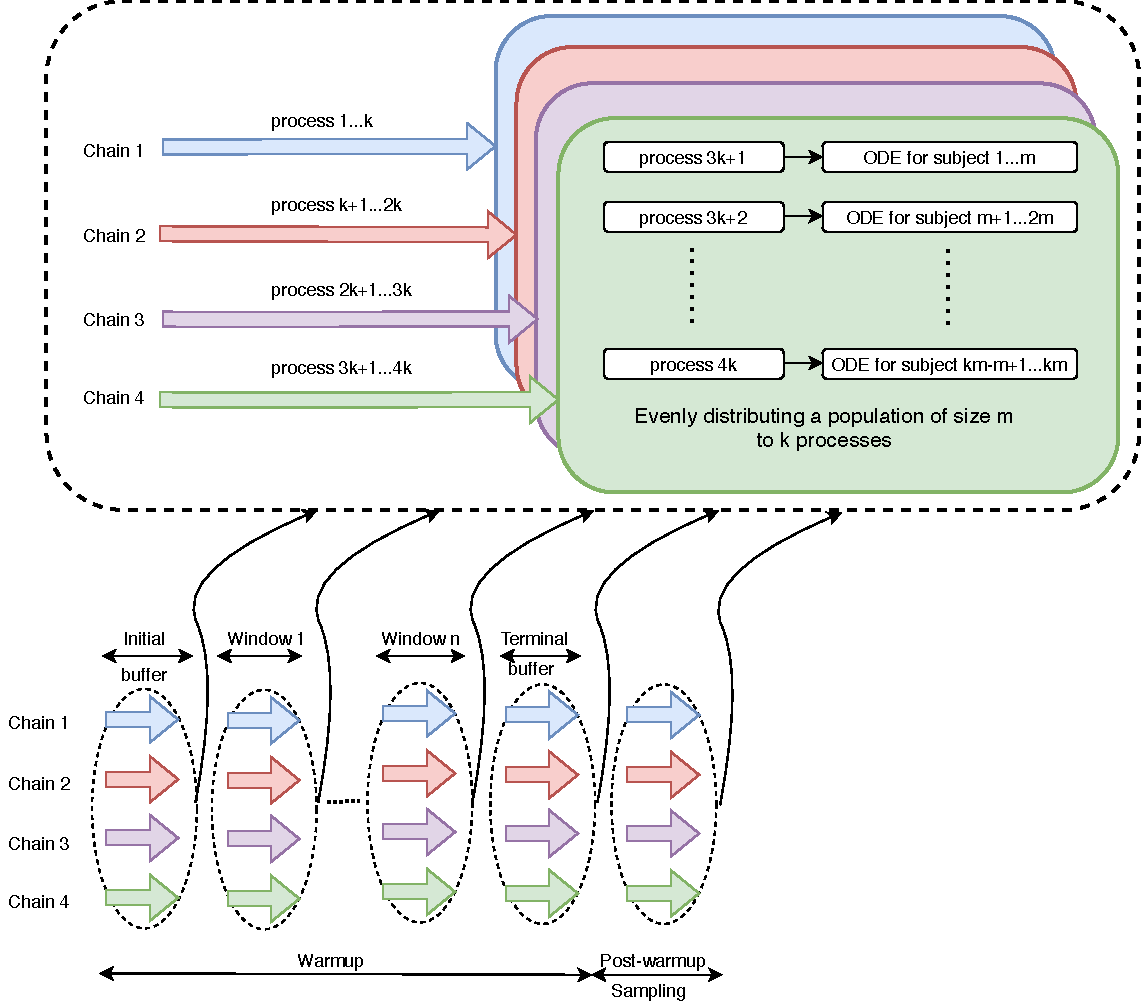
\includegraphics[width=\linewidth]{./figure/within_chain_parallel_diagram.pdf}
\captionof{figure}{Multilevel parallelism for ODE-based population models. A simplified version of Figure 1, the lower diagram shows the cross-chain warmup through multiple windows. In within-chain parallelization, as shown in the upper diagram, each chain has its own parameter samples(indicated by different colors), and dedicated processes for solving the population model. \label{multilevel-diagram}}
\end{center}

\begin{center}
\begin{tabular}{l l l}
\hline
Level & Parallel operation & Parallel communication \\
\hline
1 & parallel chains with cross-chain warmup & at the end each warmup window \\
2 & within-chain parallel group ODE solver & when likelihhood is evaluated \\
\hline
\end{tabular}
\captionof{table}{A framework of
\emph{multilevel parallelism} for Bayesian inference of population models. \label{tab:multilevel}}
\end{center}

A time-to-event model for the time to the first grade 2+ peripheral neuropathy (PN)
event in patients treated with an antibody-drug conjugate (ADC)
delivering monomethyl auristatin E (MMAE). We call it
Time-To-PN(TTPN) model, and analyze data using a
simplified version of the model reported in
\cite{lu_time--event_2017}. We consider three treatment arms:
fauxlatuzumab vedotin 1.2, 1.8 and 2.4 mg/kg IV boluses q3w x 6 doses,
with 20 patients per treatment arm. In this model,
each patient's PK is described by an effective compartment model(one-compartment),
and PD by a linear model. The likelihood for time to first 2+ PN event
is described by a hazard function that depends on the concentration
effect through Weibull distribution. Two unknowns from
PK model and the cumulative hazard form a three-component
ODE system. Each evaluation of likelihood requires solving this
3-system for every patient. 

In Torsten's model, ODEs corresponding to the entire
population can be solved by a single call of \texttt{\texttt{pmx\_solve\_group\_rk45}} function. The three parameters of the
model are:
\begin{itemize}
\item \(k_{e0}\) in effective compartment model.
\item \(\alpha\) the coefficient of linear PD model.
\item \(\beta\) Weibull distribution scale parameter.
\end{itemize}

Similar to previous section, Figure shows performance of cross-chain and
regular runs based on target ESS = 400. Unlike in previous models, we
did not performe runs with multiple seed or target ESS to avoid long
computing time. One can make conclusion consistent with the other
models, that the cross-chain warmup reduce total run time without
compromising ESS.

\begin{center}
\begin{tabular}{l l l}
\hline
 & Cross-chain & Regular \\
\hline
 \texttt{leapfrogs(warmup)}        &  \texttt{1.002225e+04}  & \texttt{1.588275e+04}\\
 \texttt{leapfrogs(sampling)}      &  \texttt{1.709250e+04}  & \texttt{1.831600e+04}\\
 \texttt{leapfrogs(warmup)/iter}   &  \texttt{1.822227e+01}  & \texttt{1.588275e+01}\\
 \texttt{leapfrogs(sampling)/iter} &  \texttt{1.709250e+01}  & \texttt{1.831600e+01}\\
 \texttt{min(bulk\_ESS/iter)}       & \texttt{2.805000e-01}  & \texttt{2.340000e-01}\\
 \texttt{min(tail\_ESS/iter)}       & \texttt{3.482500e-01}  & \texttt{3.205000e-01}\\
 \texttt{min(bulk\_ESS/leapfrog)}   & \texttt{1.641071e-02}  & \texttt{1.277572e-02}\\
 \texttt{min(tail\_ESS/leapfrog)}   & \texttt{2.037443e-02}  & \texttt{1.749836e-02}\\
 \texttt{max(elapsed\_time)}        & \texttt{1.702630e+03}  & \texttt{1.979646e+03}
\end{tabular}
\end{center}

\begin{center}
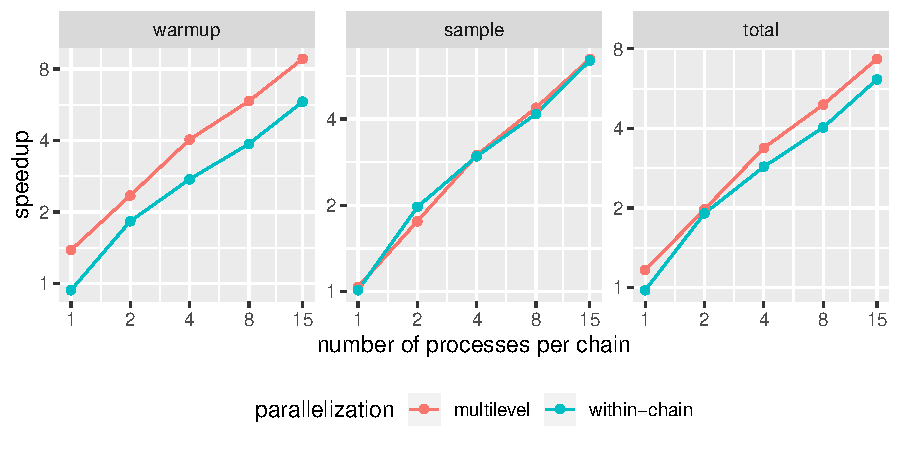
\includegraphics[width=\linewidth]{./figure/ttpn2_perf_benchmark.pdf}
\captionof{figure}{Multilevel scheme parallel performance based on TTPN model.}
\end{center}

Next, we apply multilevel method to TTPN model with a fixed target ESS
= 400, by running the model
with 4 chains using \(n_{\text{proc}} = 8, 16, 32, 60, 80\)
processes. Equivalently, there are
\(n_{\text{proc\_per\_chain}} = 2, 4, 8, 15, 20\)
processes per chain so that within-chain parallelization can be utilized.
With population size 60, each process handles solution of
\(n_{\text{id}} = 30, 15, 7, 4, 3\)
subjects' ODE system, respectively.

To show parallel scaling performance, we collect \texttt{\texttt{stanfit}} objects of the benchmark runs
and plot their wall time speedup against regular Stan runs. With all
runs having 1000 post-warmup sampling iterations, in
multilevel runs the number of warmup iterations is determinted at
runtime, while both within-chain parallel runs and regular Stan runs
have 1000 warmup iterations. Among 4 chains in a run, we use the
one with maximum total walltime(in seconds) as performance measure, as
in practice usually further model evaluation becomes accessible only
after all chains finish.

As shown in Figure \ref{cc-diagram}, both muiltilevel and
within-chai-only parallel runs exhibit good scaling up to 60
processes(15 processes per chain \(\times\) 4 chains)


\end{multicols}
\vspace{0.5em}
}

%----------------------------------------------------------------------------------------
%	CONCLUSION
%----------------------------------------------------------------------------------------

\headerbox{Conclusion and future work}{name=conclusion,column=2,below=multilevel,above=bottom}{
Multilevel parallelism using in Stan and Torsten
significantly improves computational efficiency and extends
the range of models that may be practically implemented. A natual
follow-up of this study is to seek higher efficiency by maintaining
target ESS while increasing the number of parallel chains during warmup.
}

%----------------------------------------------------------------------------------------
%	REFERENCES
%----------------------------------------------------------------------------------------

\headerbox{References}{name=references,column=3,above=bottom,aligned=conclusion}{

\renewcommand{\section}[2]{\vskip 0.05em} % Get rid of the default "References" section title
\small{ % Reduce the font size in this block
\bibliographystyle{siam}
\bibliography{torsten} % Use torsten.bib as the bibliography file
}}

%----------------------------------------------------------------------------------------
%	CONTACT INFORMATION
%----------------------------------------------------------------------------------------

% \headerbox{Contact Information}{name=contact,column=3,aligned=references,above=bottom}{ % This block is as tall as the references block

% \begin{description}\compresslist
% \item[Web] www.university.edu/smithlab
% \item[Email] john@smith.com
% \item[Phone] +1 (000) 111 1111
% \end{description}
% }




%----------------------------------------------------------------------------------------

\end{poster}

\end{document}
